\documentclass[12pt,]{article}
\usepackage[utf8]{inputenc}
\usepackage[T1]{fontenc}
\usepackage{mathptmx}
\usepackage{geometry}
\usepackage{mathtools}
\usepackage[english]{babel}
\usepackage{graphicx}
\usepackage{subcaption}
\usepackage{stackengine}
\usepackage[os=win]{menukeys}
\usepackage{hyperref}
\usepackage{minted}
\usepackage{xcolor}
\usepackage{tikz}
\usepackage[yyyymmdd,hhmmss]{datetime}
\usepackage{etoolbox}
\usepackage[inline]{enumitem}
\usepackage{pdfpages}

\newcommand{\WindowsLogo}{\raisebox{-0.1em}{
\includegraphics[height=0.8em]{images/logo/Windows_3_logo_simplified}}}
%\newcommand{\PowerLogo}{\raisebox{-0.1em}{
\includegraphics[height=0.8em]{images/logo/power}}}
\newcommand{\WinKey}{\keys{\WindowsLogo}}
\newcommand{\PowerKey}{\keys{\PowerLogo}}

\patchcmd{\thebibliography}{\section*{\refname}}{}{}{}

\newcommand{\ShowOsVersion}{
	\immediate\write18{\unexpanded{foo=`uname -sro` && echo "${foo}" > tmp.tex}}
	\input{tmp}\immediate\write18{rm tmp.tex}
}

\newcommand{\ShowTexVersion}{
	\immediate\write18{\unexpanded{foo=`pdflatex -version | head -n1 | cut -d' ' -f1,2` && echo "${foo}" > tmp.tex}}
	\input{tmp}\immediate\write18{rm tmp.tex}
}

\addto\captionsenglish{\renewcommand{\contentsname}{Daftar Isi}}
\addto\captionsenglish{\renewcommand{\figurename}{Gambar}}

\hypersetup{
	colorlinks=true, %set true if you want colored links
	linktoc=all,     %set to all if you want both sections and subsections linked
	linkcolor=blue,  %choose some color if you want links to stand out
	urlcolor=blue,   %url color
}

\geometry{
	a4paper,
	left=10mm,
	right=10mm,
	top=10mm,
	bottom=15mm,
}

\title{\LARGE \bf
	Laporan Pengujian Unit Prototype Portable/Handheld Audiometri\\
}

\author{Achmadi ST MT}

\date{}

\hypersetup{citecolor=black}

\definecolor{LightGray}{gray}{0.95}

%\pagecolor[rgb]{0.1,0.1,0.1}
%\color[rgb]{1,1,1}

\begin{document}
	\thispagestyle{empty}

	\begin{titlepage}
		\centering
		\vfill
		\vfill
		\maketitle
		\vfill
		
\includegraphics[width=200pt]{images/logo/logoviblab}
		\vfill
		\vfill
		Update: {\today} \currenttime \\
	\end{titlepage}

	%%%%%%%%%%%%%%%%%%%%%%%%%%%%%%%%%%%%%%%%%%%%%%%%%%%%%%%%%%%%%%%%%

	\newpage
	\tableofcontents

	%%%%%%%%%%%%%%%%%%%%%%%%%%%%%%%%%%%%%%%%%%%%%%%%%%%%%%%%%%%%%%%%%

	\newpage
	\section{Pendahuluan}

	\subsection{Tujuan Pengujian}

	Tujuan Pengujian disini adalah untuk mengetahui nilai aktual \textit{loudness} output dalam dB (SPL).

	\subsection{Waktu dan Tempat Pengujian}

	Seluruh pengujian di lakukan di Ruang Un-Echoic Chamber Laboratorium Fisika Bangunan Teknik Fisika
	Institut Teknologi Bandung. Waktu pengujian adalah minggu kedua di bulan Desember 2020.

	\subsection{Batasan Pengujian}

	Batasan pengujian adalah sebagai berikut:

	\begin{enumerate}
		\item Nilai frekuensi dan konsistensi frekuensi tidak diukur di ruang Unechoic chamber tersebut di atas
		karena telah diuji selama proses pengembangan dan perakitan unit prototype dan telah terbukti konsisten pada nilai yang diinginkan.

		\item Pengujian tidak dilakukan pada tubuh manusia sebenarnya melainkan menggunakan manekin yang diproduksi oleh GRASS KEMAR.
	\end{enumerate}

	%%%%%%%%%%%%%%%%%%%%%%%%%%%%%%%%%%%%%%%%%%%%%%%%%%%%%%%%%%%%%%%%%

	\newpage
	\section{Metode Pengujian}

	\subsection{Persiapan}

	Berikut adalah perangkat keras yang perlu disiapkan untuk pengujian ini:

	\begin{itemize}

		\item Unit Prototype Audiometri yang akan diuji.

		Pastikan unit prototype masih normal sebagaimana pada bab sebelumnya.

		\begin{figure}[!ht]
			\centering
			\begin{subfigure}[b]{0.3\textwidth}
				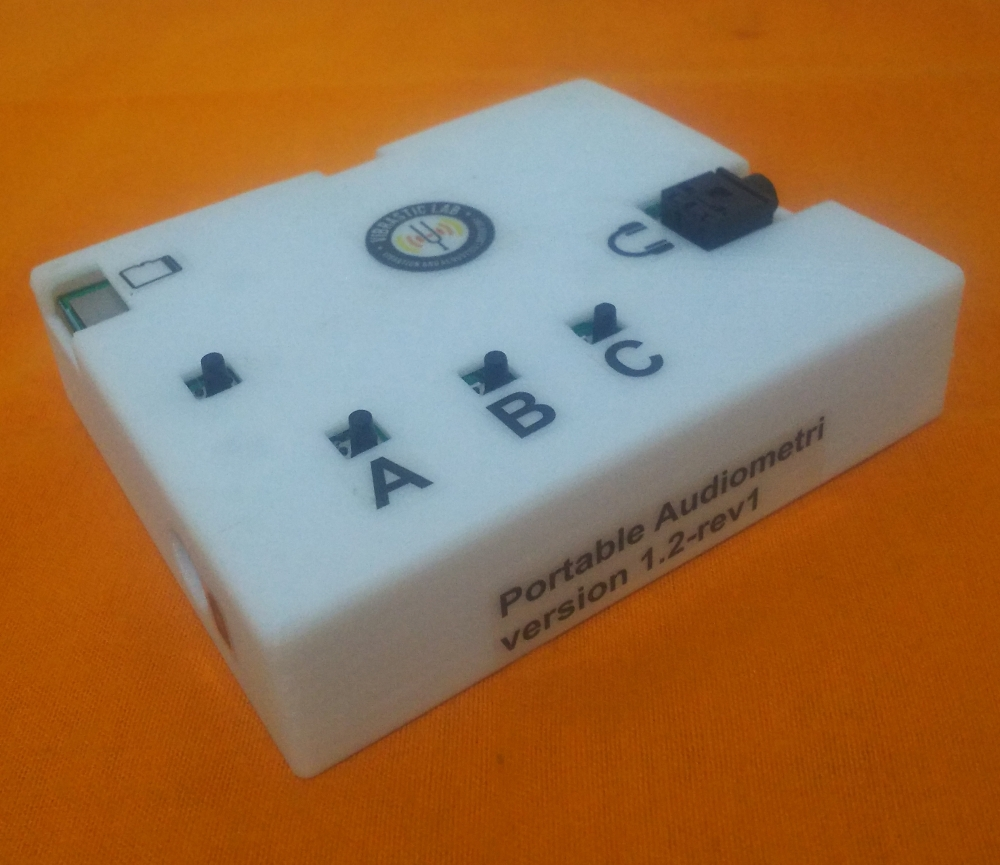
\includegraphics[width=\textwidth]{images/foto/unit}
				\caption{Unit Prototype}
			\end{subfigure}
			\begin{subfigure}[b]{0.3\textwidth}
				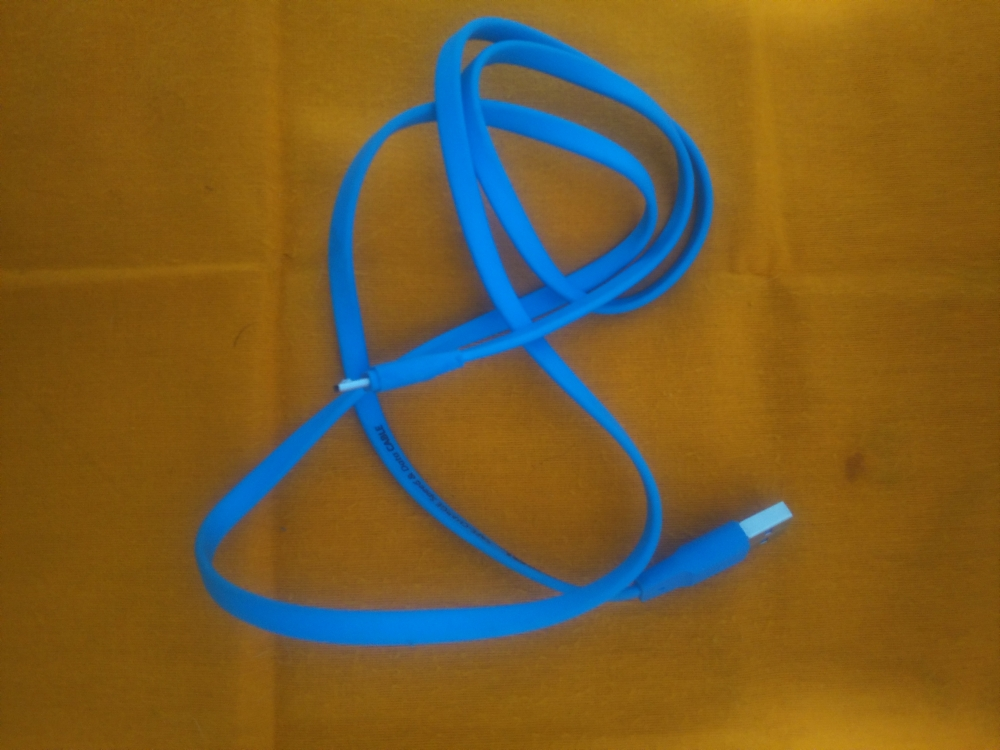
\includegraphics[width=\textwidth]{images/foto/kabel}
				\caption{Kabel USB}
			\end{subfigure}
			\caption{Prototype}
		\end{figure}


		\item Wired-Headphone dengan impedansi tiap channel antara $32\Omega$ hingga $300\Omega$

		Headphone yang digunakan disini adalah:
		\begin{itemize}
			\item Headphone Miniso (tanpa active noise cancelling)
			\item Headphone BOSE (dilengkapi active noise cancelling)
		\end{itemize}
		\begin{figure}[!ht]
			\centering
			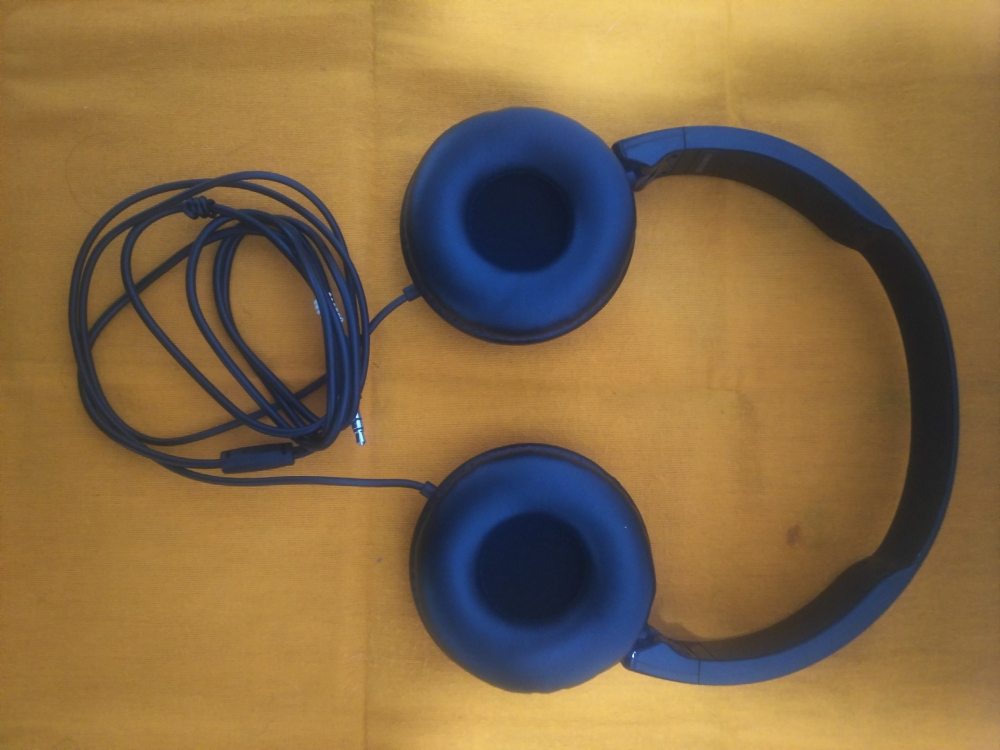
\includegraphics[width=200pt]{images/foto/phone}
			\caption{Wired Headphone}
		\end{figure}

		\newpage
		\item Kalibrasi Mikrofon pada manekin KEMAR menggunakan \textit{tone generator} yang tersedia pada paket GRASS KEMAR.
		Kemudian pasang Headphone pada manekin.
		\begin{figure}[!ht]
			\centering
			\begin{subfigure}[b]{0.3\textwidth}
				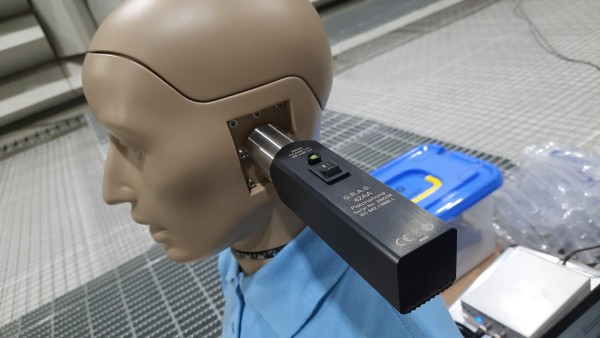
\includegraphics[width=\textwidth]{images/foto/calib}
				\caption{Kalibrasi Mikrofon}
			\end{subfigure}
			\begin{subfigure}[b]{0.3\textwidth}
				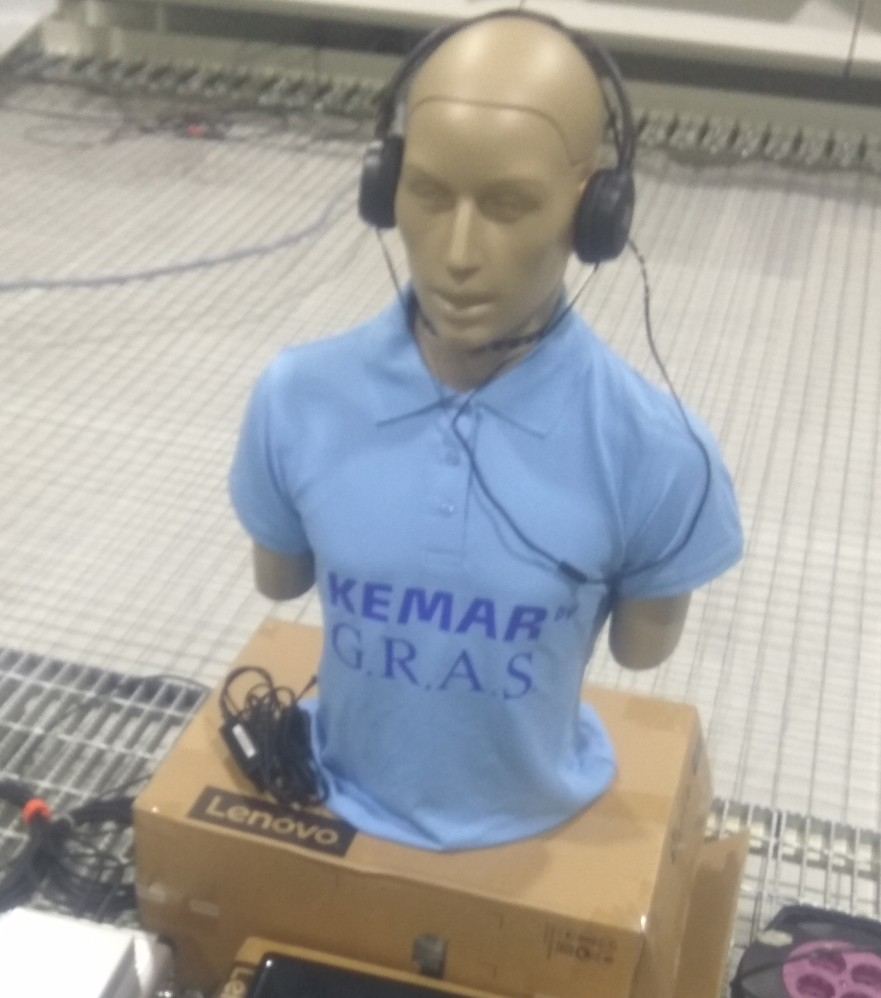
\includegraphics[width=\textwidth]{images/foto/kemar}
				\caption{Headphone Terpasang}
			\end{subfigure}
			\caption{GRASS KEMAR}
		\end{figure}

	\end{itemize}

	\subsection{Audio Analyzer}

	Mikrofon GRASS KEMAR dihubungkan dengan Audio-Box dan data Audio digital dikumpulkan dengan perangkat lunak Real-Time Analyzer via USB.
	Perangkat lunak ini merupakan bagian dari paket software DSFF3 buatan Yoshimasha.

	\begin{figure}[!ht]
		\centering
		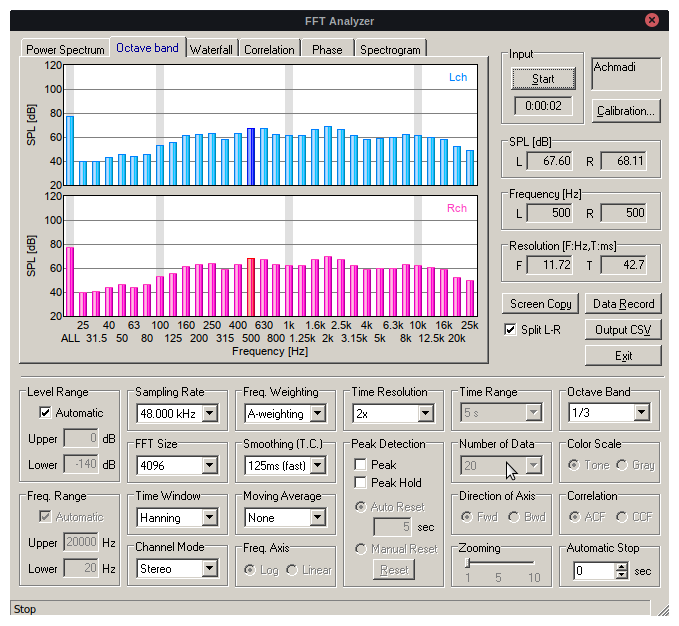
\includegraphics[width=300pt]{images/kemar/fft}
		\caption{Tampilan Audio Analyzer}
	\end{figure}

	\newpage
	\subsection{Teknis Pengujian}

	Berikut langkah proses pengujian

	\begin{itemize}
		\item Nyalakan unit prototype dan sambungkan USB protype ke komputer.
		\begin{figure}[!ht]
			\centering
			\begin{subfigure}[b]{0.3\textwidth}
				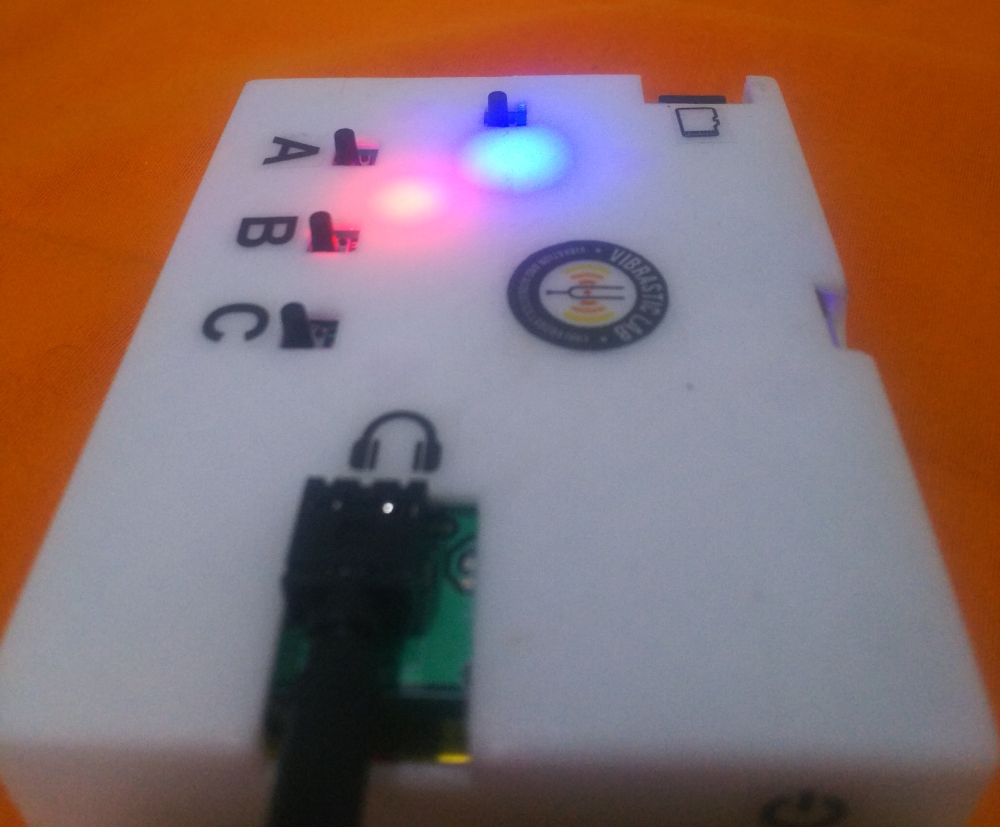
\includegraphics[width=\textwidth]{images/foto/standby}
				\caption{Prototype Standby}
			\end{subfigure}
			\begin{subfigure}[b]{0.3\textwidth}
				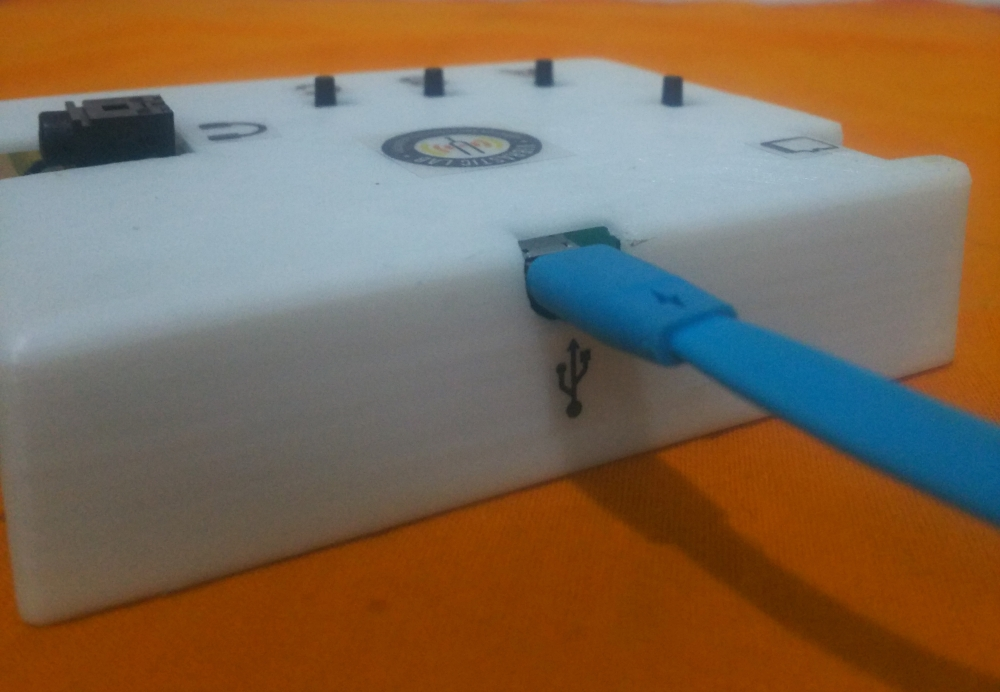
\includegraphics[width=\textwidth]{images/foto/konek}
				\caption{USB Terpasang}
			\end{subfigure}
			\caption{Menyalakan Unit Prototype}
		\end{figure}


		\item Akses prototype menggunakan serial port (semisal Hercules.exe) pada komputer.
		\begin{figure}[!ht]
			\centering
			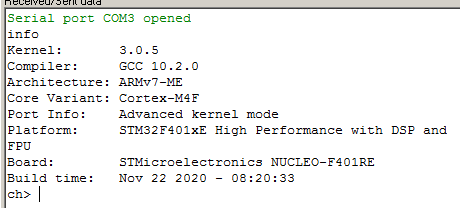
\includegraphics[width=300pt]{images/terminal/hercules_text}
			\caption{Contoh respon serial port}
		\end{figure}

		\item Perintah Serial untuk membangkitkan tone
		Perintah untuk membangkitkan tone dengan frekuensi dan skala yang diinginkan selama 5detik.

		Pola perintah serialnya adalah:
		\begin{minted}[frame=lines,framesep=2mm,fontsize=\small]{text}
out <frekuensi> <amplitudo>
		\end{minted}

		dengan:
		\begin{itemize}

			\item frekuensi adalah nilai frekuensi (dalam Hz) mulai 250, 500, 1000, 2000, 4000, dan 8000.

			\item amplitudo adalah skala amplitudo pada nilai 1, 2, 3, 4, 5, 6, 7, 8, dan 9.

		\end{itemize}

		Contoh untuk tone 500Hz pada skala amplitudo 6 (diakhiri (\keys{\return})):
		\begin{minted}[frame=lines,framesep=2mm,fontsize=\small]{text}
out 500 6
		\end{minted}

		\newpage
		Maka salah satu channel headphone yang terhubung prototype akan membangkitkan tone selama 5 detik.

		\begin{figure}[!ht]
			\centering
			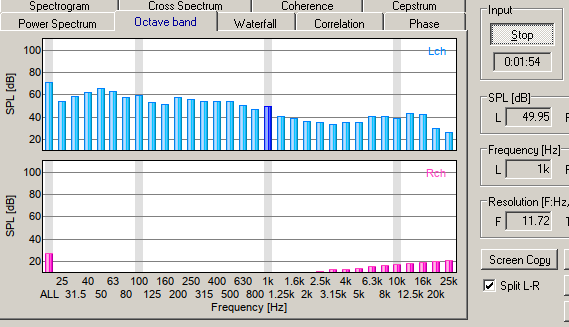
\includegraphics[width=300pt]{images/terminal/contoh}
			\caption{Contoh Nilai Uji}
		\end{figure}

		\item Hasil yang diinginkan adalah tabel dengan spesifikasi berikut:
		\begin{itemize}
			\item tabel background noise terhadap waktu dengan KEMAR tanpa headphone (1 tabel).
			\item tabel background noise terhadap waktu dengan KEMAR menggunakan kedua headphone, yaitu BOSE dan Miniso (2 tabel).
			\item tabel loudness output di setiap frekuensi untuk setiap kenaikan skala amplitudo, untuk 2 prototype dengan 2 headphone, masing 3 tabel per hari.
			\item tabel loudness output di setiap frekuensi untuk setiap penurunan skala amplitudo, untuk 2 prototype dengan 2 headphone, masing 3 tabel per hari.
			\item pengukuran loudness output dilakukan di 3 hari berbeda.
		\end{itemize}

		sehingga diharapkan total 75 tabel hasil pengukuran.
	\end{itemize}

	\newpage
	\section{Hasil Pengujian}

	\subsection{Tabel Hasil}

	Tabel hasil pengujian cukuk banyak yang akan memakan tempat disini sehingga disediakan tempat di repository pemrograman Lab Vibrastic pada tautan berikut:\\
	\url{https://github.com/VibrasticLab/pikoakustik/tree/stm32f401re_3pin/document/hasil_ukur_lanjutan/tabel_hasil_ukur}.\\

	Untuk kemudahan dalam pengolahan, tersedia pula tabel data tersebut dalam format Python Numpy array yang dapat diakses di tautan:\\
	\url{https://github.com/VibrasticLab/pikoakustik/blob/stm32f401re_3pin/document/hasil_ukur_lanjutan/python/itb_data_pool.py}\\

	Kemudian untuk memudahkan proses pengolahan data, digunakan pula perangkat lunak Jupyter Note yang berkasnya dapat diakses di tautan:\\
	\url{https://github.com/VibrasticLab/pikoakustik/blob/stm32f401re_3pin/document/hasil_ukur_lanjutan/python/itb_data_pool.py}\\

	\subsection{Pengolahan Data}

	Pengolahan data hasil pengujian dikelompokkan pada 3 topik, yaitu loudness, efek histeresis, dan efek perbedaan hari.

	\subsubsection{Loudness}

	Untuk pengolahan data terkait loudness, terbagi dalam dua topik, yaitu loudness terendah dan model matematis skala loudness

	\begin{itemize}
		\item \textbf{Loudness Terendah.}\\

		Berikut adalah grafik \textit{surface} pengukuran bising lingkungan:

		\begin{figure}[!ht]
			\centering
			\begin{subfigure}[b]{0.3\textwidth}
				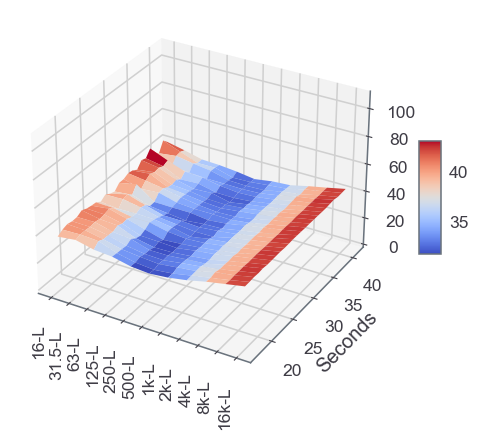
\includegraphics[width=\textwidth]{images/graph/nounitnohp}
				\caption{Tanpa Headphone}
			\end{subfigure}
			\begin{subfigure}[b]{0.3\textwidth}
				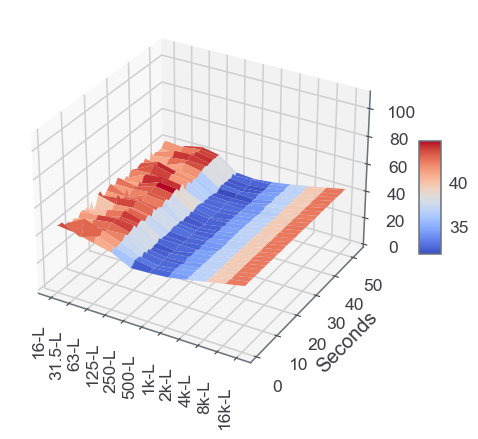
\includegraphics[width=\textwidth]{images/graph/nounitminiso}
				\caption{Headphone Miniso}
			\end{subfigure}
			\begin{subfigure}[b]{0.3\textwidth}
				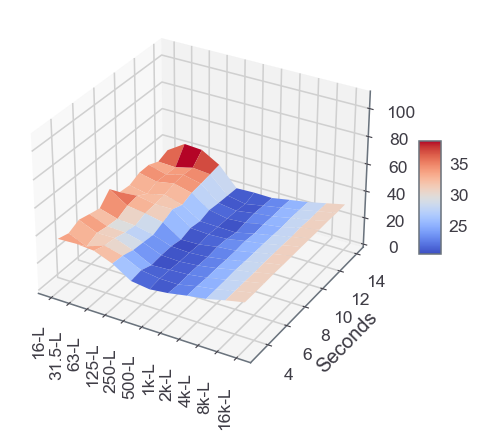
\includegraphics[width=\textwidth]{images/graph/nounitbose}
				\caption{Headphone BOSE}
			\end{subfigure}
			\caption{Bising Lingkungan}
		\end{figure}

		Dengan melihat skala \textit{colormap} grafik di atas terlihat bahwa headphone BOSE memiliki taraf bising paling rendah.
		Hal ini dikarenakan selain memiliki peredam bising pasif dengan struktur headphone yang melingkupi telinga secara penuh,
		juga tersedia fitur peredam bising aktif yang membatalkan bising lingkungan masuk ke mikrofon.

		\newpage
		Selanjutnya berikut adalah grafik nada terendah di setiap frekuensi dibandingkan bising lingkungan 3 detik pertama pada setiap frekuensi:

		\begin{figure}[!ht]
			\centering
			\begin{subfigure}[b]{0.5\textwidth}
				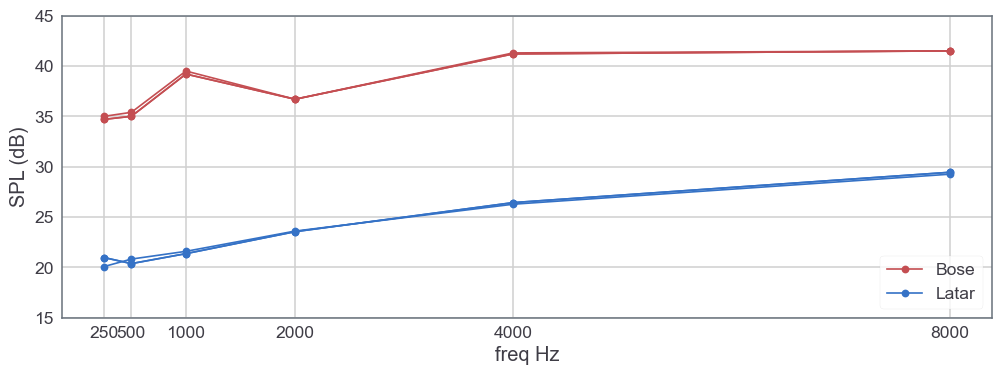
\includegraphics[width=\textwidth]{images/graph/boselowest_unit1}
				\caption{Prototype A}
			\end{subfigure}
			\begin{subfigure}[b]{0.5\textwidth}
				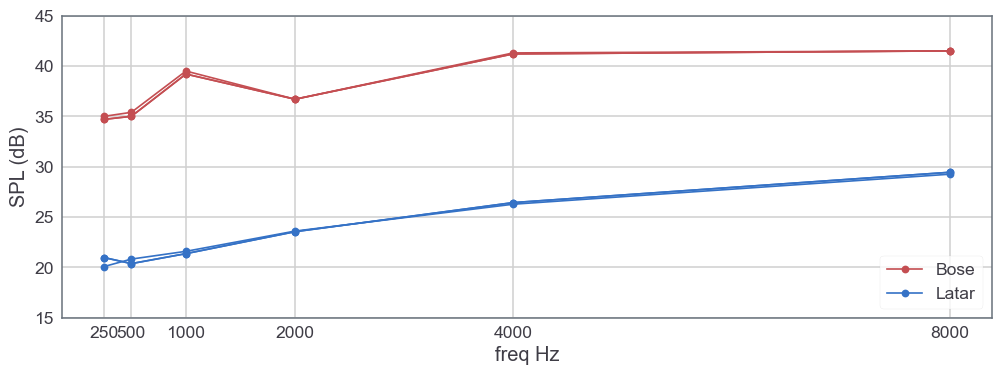
\includegraphics[width=\textwidth]{images/graph/boselowest_unit1}
				\caption{Prototype B}
			\end{subfigure}
			\caption{Nada terendah BOSE terhadap bising lingkungan}
		\end{figure}

		\begin{figure}[!ht]
			\centering
			\begin{subfigure}[b]{0.5\textwidth}
				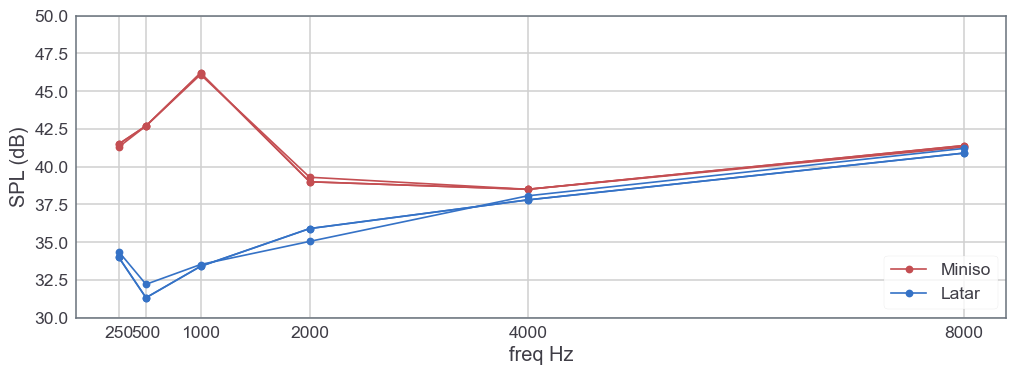
\includegraphics[width=\textwidth]{images/graph/minisolowest_unit1}
				\caption{Prototype A}
			\end{subfigure}
			\begin{subfigure}[b]{0.5\textwidth}
				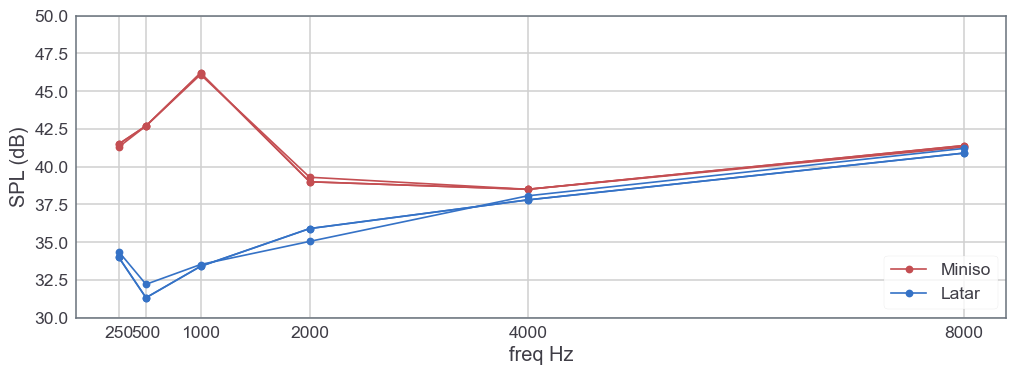
\includegraphics[width=\textwidth]{images/graph/minisolowest_unit1}
				\caption{Prototype B}
			\end{subfigure}
			\caption{Nada terendah Miniso terhadap bising lingkungan}
		\end{figure}

		\begin{figure}[!ht]
			\centering
			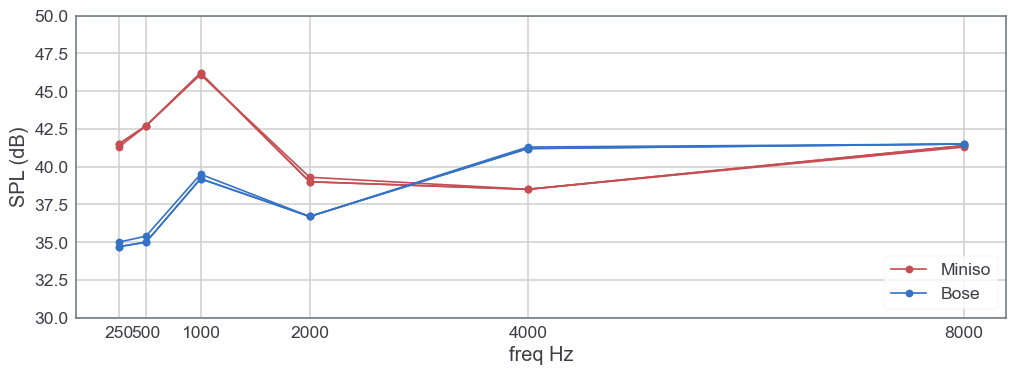
\includegraphics[width=300pt]{images/graph/lowestbosevsminiso}
			\caption{Nada terendah BOSE vs Miniso}
		\end{figure}

		\newpage
		Berdasarkan grafik di atas, dapat disimpulkan bahwa penggunaan headphone BOSE dianggap lebih baik
		dibandingkan Miniso dengan pertimbangan:
		\begin{enumerate}
			\item Loudness terendah BOSE cenderung lebih rendah dibandinhkan Miniso.
			\item Loudness terendah Miniso cenderung tenggelam pada bising lingkungan.
		\end{enumerate}

		Untuk selanjutnya, pengolahan data hanya difokuskan pada BOSE Headphone yang direncanakan akan
		digunakan sebagai default headphone.

		\item \textbf{Model skala loudness.}

		Dengan merata-rata seluruh matrix tabel didapat matrix untuk prototype Unit A sebagai berikut:

		\[\left[
		\begin{matrix}
			34.9 & 36.4 & 40. &  44.6 & 52. &  56.1 & 62.1 & 68.2 & 74.2\\
			35.3 & 37.4 & 41.4 & 46.6 & 52.2 & 58.2 & 64.2 & 70.3 & 76.4\\
			39.2 & 42.4 & 47. & 52.5 & 58.3 & 64.3 & 70.3 & 76.4 & 82.4\\
			36.8 & 38.2 & 41.2 & 45.8 & 51.2 & 57.2 & 63.2 & 69.3 & 75.3\\
			41.4 & 44. &  48.2 & 53.4 & 59.2 & 65.1 & 71.2 & 77.2 & 83.2\\
			42. &  43.1 & 45.9 & 50.2 & 55.7 & 61.5 & 67.5 & 73.5 & 79.6\\
		\end{matrix}
		\right]\]

		Kemudian dengan memperhatikan pola grafik tiap frekuensi (baris) pada matrix unit A:
		\begin{figure}[!ht]
			\centering
			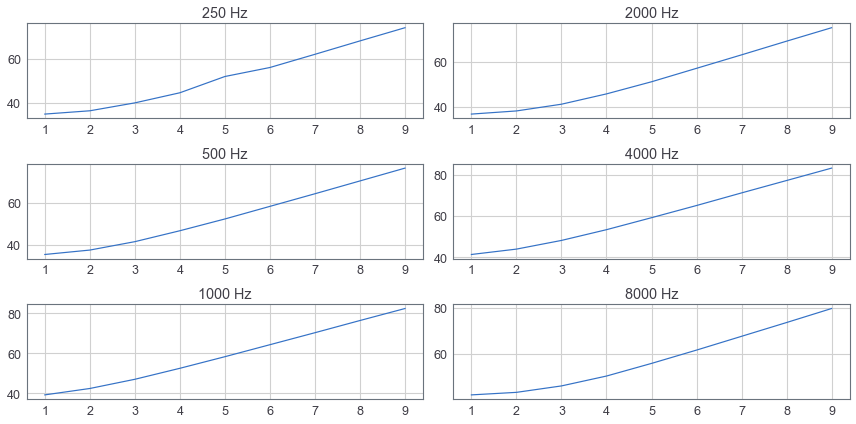
\includegraphics[width=400pt]{images/graph/boseprotoA}
			\caption{Grafik loudness setiap frekuensi}
		\end{figure}

		Pendekatan model matematis untuk loudness terhadap skala input menggunakan polynomial:\\
		\[f(x) = ax^3 + bx^2 + cx + d\]

		Estimasi model menggunakan perangkat lunak Numpy Polyfit yang tersedia di Python.
		Hasil estimasi untuk prototype A pada setiap frekuensi.

		\[f_{250}(x) = -0.05x^3 + 1.03bx^2 - 0.59cx + 34.21\]
		\[f_{500}(x) = -0.05x^3 + 0.93bx^2 + 0.09cx + 34.15\]
		\[f_{1000}(x) = -0.04x^3 + 0.69bx^2 + 1.72cx + 36.69\]
		\[f_{2000}(x) = -0.06x^3 + 1.15bx^2 - 1.58cx + 37.22\]
		\[f_{4000}(x) = -0.04x^3 + 0.85bx^2 + 0.68cx + 39.78\]
		\[f_{8000}(x) = -0.06x^3 + 1.2bx^2 - 1.99cx + 42.79\]

		Model matematis ini yang akan di implementasikan ke prototype.

		\newpage
		Selanjutnya untuk prototype B, dilakukan metode perhitungan yang sama.

		Berikut matrix rata-rata loudness pengukuran:

		\[\left[
		\begin{matrix}
			34.8&36.&39.8&44.6&49.9&55.8&61.9&68.&74.&\\

			35.2&37.2&41.2&46.4&52.&58.&64.1&70.2&76.2\\

			38.9&42.1&46.8&52.2&58.&64.&70.1&76.1&82.1\\

			36.7&38.&41.&45.5&51.&56.9&63.&69.&75.1\\

			41.3&43.8&47.9&53.2&59.&64.9&70.9&77.&83.&\\

			41.8&43.&45.6&49.8&55.2&61.&67.&73.&79.&\\
		\end{matrix}
		\right]\]

		Hasil estimasi untuk prototype B pada setiap frekuensi.

		\[f_{250}(x) = -0.05x^3 + 1.08bx^2 - 1cx + 34.56\]
		\[f_{500}(x) = -0.05x^3 + 0.98bx^2 - 0.12cx + 34.21\]
		\[f_{1000}(x) = -0.04x^3 + 0.69bx^2 + 1.74cx + 36.38\]
		\[f_{2000}(x) = -0.06x^3 + 1.17bx^2 - 1.69cx + 37.21\]
		\[f_{4000}(x) = -0.04x^3 + 0.87bx^2 + 0.55cx + 39.77\]
		\[f_{8000}(x) = -0.06x^3 - 2.06bx^2 - 1.99cx + 42.73\]

		Terakhir, jika diselisih matrix koefisien didapat matrix bernilai kecil:

		\[\left[
		\begin{matrix}
			0.  & -0.05 &  0.41 & -0.35\\
			0.  & -0.05 &  0.21 & -0.06\\
			0.  &  0.   & -0.02 &  0.31\\
			0.  & -0.02 &  0.11 &  0.01\\
			0.  & -0.02 &  0.13 &  0.01\\
			0.  &  0.01 &  0.07 &  0.06\\
		\end{matrix}
		\right]\]

		dimana ini menunjukkan bahwa kedua prototype yang diuji saling identik dan saling representatif.
	\end{itemize}

	\subsubsection{Efek Histeresis}

	Selanjutnya, dengan menghitung standar deviasi di setiap elemen matrix hasil (setiap loudness dan frekuensi) sebagai array,
	didapat matriks standar deviasi di setiap unit prototype di setiap hari untuk headphone BOSE sebagai berikut:

	\begin{enumerate}
		\item Unit A. Diurut dari kiri atas, hari-1, hari-2, dan hari-3
		\[ \left( \begin{matrix}
			0.2&0.3&0.2&0.2&11.8&0.1&0.1&0.&0.1\\

			0.2&0.&0.2&0.1&0.&0.&0.&0.1&0.&\\

			0.1&0.1&0.&0.&0.&0.&0.&0.&0.&\\

			0.&0.&0.1&0.1&0.1&0.&0.&0.&0.&\\

			0.1&0.1&0.1&0.&0.&0.&0.&0.&0.&\\

			0.1&0.1&0.1&0.1&0.&0.&0.&0.&0.&\\
		\end{matrix} \right)
		%
		\left( \begin{matrix}
			0.1&0.1&0.2&0.1&0.1&0.&0.&0.&0.&\\

			0.1&0.1&0.1&0.1&0.1&0.&0.&0.&0.&\\

			0.1&0.1&0.&0.&0.&0.&0.&0.&0.&\\

			0.1&0.1&0.1&0.1&0.&0.&0.&0.&0.&\\

			0.1&0.1&0.1&0.&0.&0.&0.&0.&0.&\\

			0.1&0.1&0.1&0.1&0.&0.&0.&0.&0.&\\
		\end{matrix} \right)
		\]

		\[\left[
		\begin{matrix}
			0.1&0.2&0.2&0.1&0.2&0.&0.&0.&0.&\\

			0.2&0.1&0.1&0.1&0.1&0.1&0.&0.&0.&\\

			0.1&0.1&0.1&0.&0.&0.&0.&0.&0.&\\

			0.1&0.1&0.1&0.1&0.&0.&0.&0.&0.&\\

			0.2&0.1&0.1&0.&0.&0.&0.&0.&0.&\\

			0.1&0.&0.1&0.&0.1&0.&0.&0.&0.&\\
		\end{matrix}
		\right]\]

		\newpage
		\item Unit B, Diurut dari kiri atas, hari-1, hari-2, dan hari-3

		\[ \left( \begin{matrix}
			0.3&0.1&0.2&0.1&0.1&0.1&0.&0.&0.&\\

			0.2&0.1&0.1&0.1&0.1&0.&0.&0.1&0.&\\

			0.1&0.1&0.1&0.1&0.&0.&0.&0.&0.&\\

			0.1&0.1&0.1&0.&0.1&0.&0.&0.&0.&\\

			0.1&0.1&0.1&0.&0.&0.&0.&0.&0.&\\

			0.1&0.1&0.1&0.1&0.&0.&0.&0.&0.&\\
		\end{matrix} \right)
		%
		\left( \begin{matrix}
			0.1&0.2&0.2&0.2&0.1&0.1&0.&0.1&0.1\\

			0.2&0.1&0.1&0.1&0.1&0.&0.&0.&0.&\\

			0.1&0.1&0.1&0.1&0.&0.&0.&0.&0.&\\

			0.1&0.1&0.1&0.1&0.1&0.&1.1&0.&0.&\\

			0.1&0.1&0.1&0.1&0.&0.&0.&0.&0.&\\

			0.1&0.1&0.1&0.1&0.&0.&0.&0.&0.&\\
		\end{matrix} \right)
		\]

		\[\left[
		\begin{matrix}
			0.1&0.2&0.1&0.1&0.1&0.1&0.1&0.&0.&\\

			0.&0.4&0.2&0.2&0.&0.&0.&0.&0.&\\

			0.2&0.1&0.&0.&0.1&0.&0.&0.&0.&\\

			0.1&0.1&0.&0.1&0.&0.&0.&0.&0.&\\

			0.1&0.1&0.1&0.&0.&0.&0.&0.&0.&\\

			0.1&0.1&0.&0.&0.&0.&0.&0.&0.&\\
		\end{matrix}
		\right]\]

	\end{enumerate}

	Dengan memperhatikan matrix standar deviasi di atas, dapat terlihat bahwa output loudness cenderung konsisten
	baik terkait efek histeresis maupun perbedaan hari pengukuran.

	\newpage
	\section{Lampiran}

	\subsection{Notebook Olah Data}
	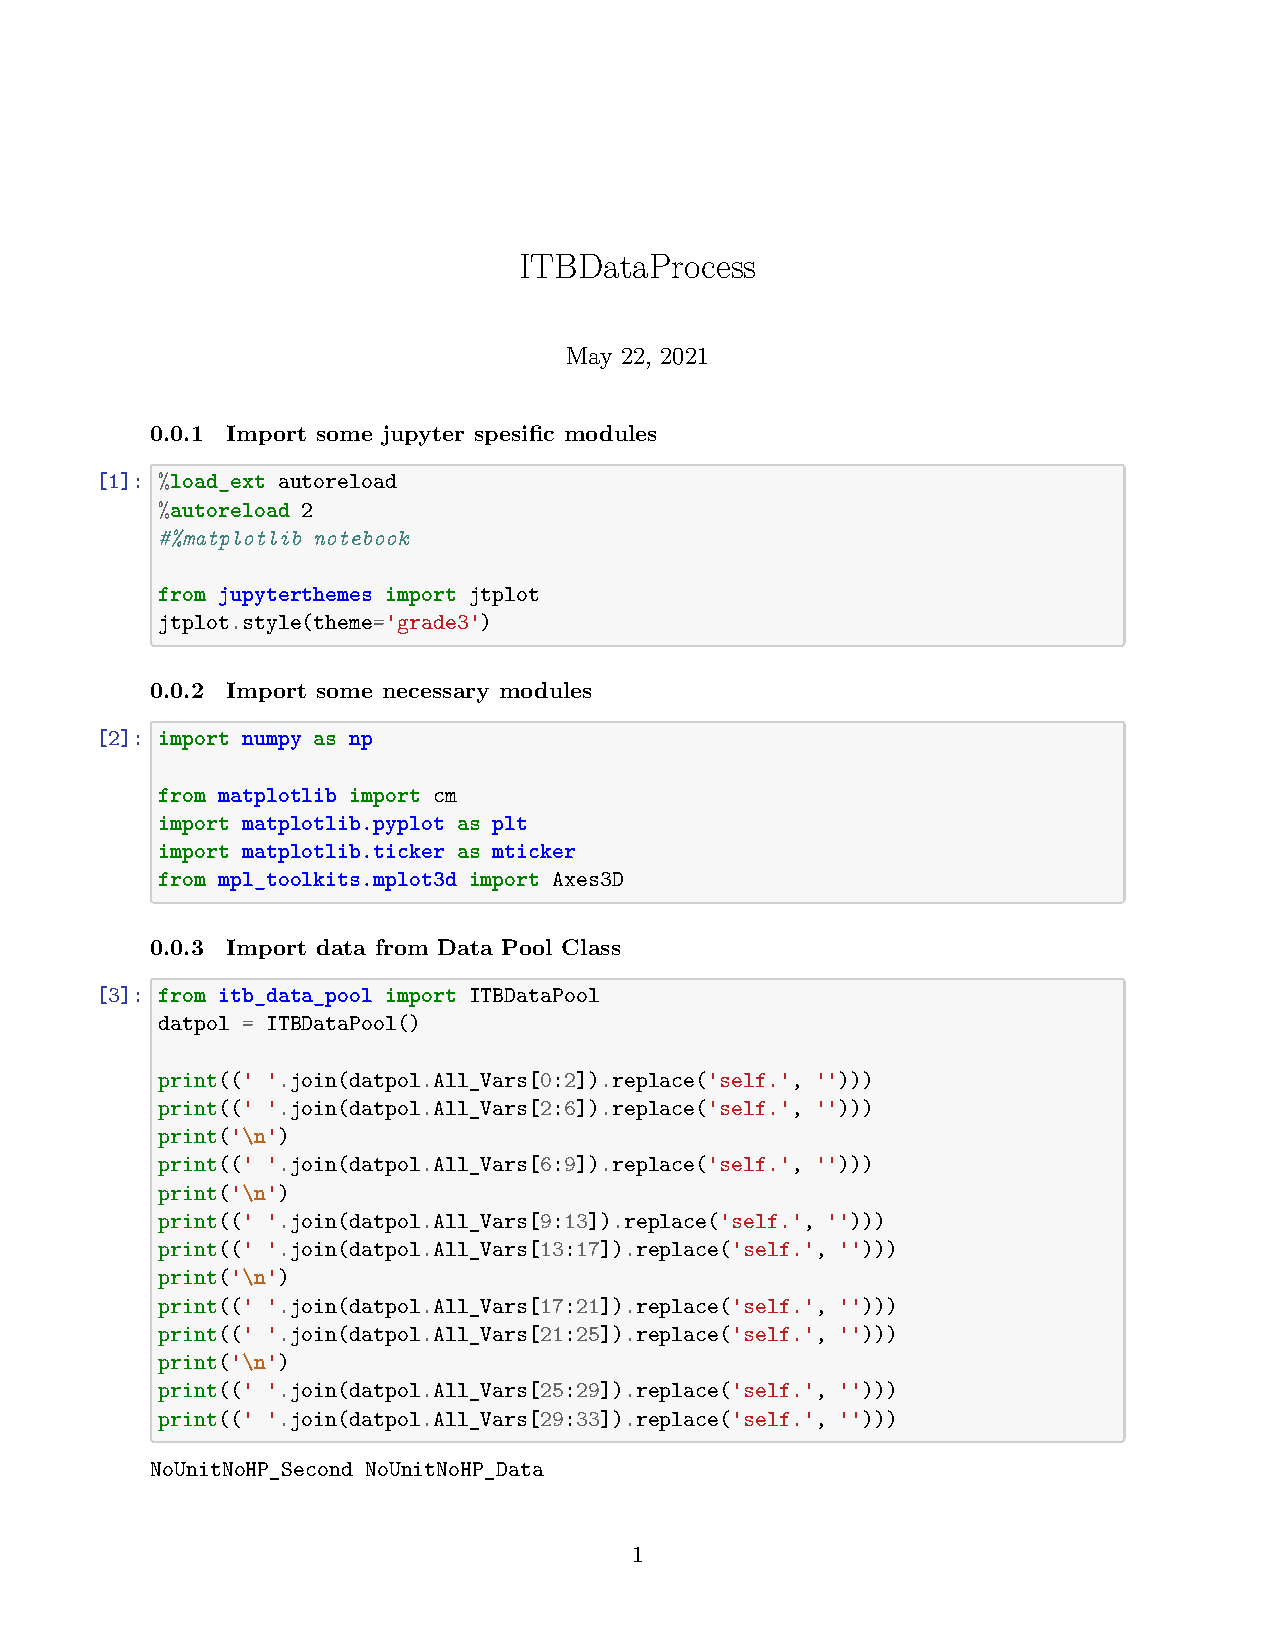
\includepdf[pages=-]{python/ITBDataProcess.pdf}

\end{document}
